\section{光滑曲线的第一个要求}

对于好函数的要求——光滑,我们第一个直觉是“不能断”。

\begin{figure}[h]
\centering
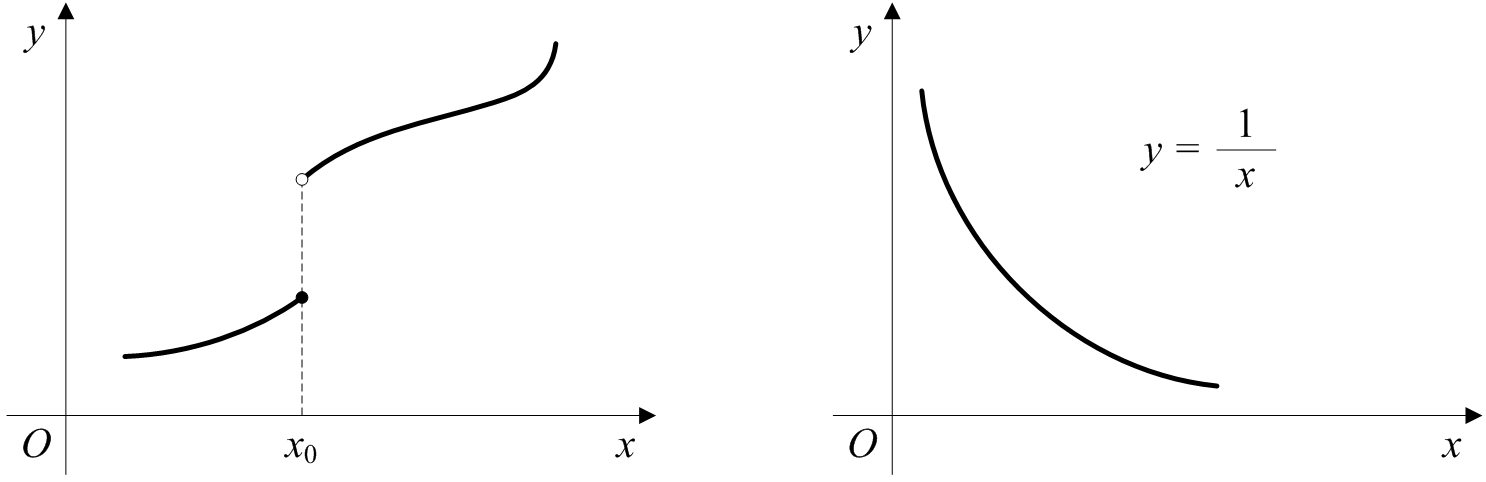
\includegraphics[height=3cm]{1.2.png}
\end{figure}

左上图的曲线不光滑,它“断了”。
右上图的曲线咋看没问题,但是在$x=0$处断了,不是人为地断,而是这个函数根本到不了断点。

那么什么是断,什么又不是断,我们需要给出一个数学上的“不断”的定义——连续。




